\documentclass{article}
\usepackage{geometry}
\usepackage[pdftex]{graphicx}
\usepackage[utf8]{inputenc}
\usepackage{algorithmic}
\usepackage{algorithm}
\usepackage{titlesec}
\usepackage{float}
\usepackage{amsthm}
\usepackage{enumitem}

\newtheorem{mydef}{Definition}

\begin{document}

\title{Paper Review: Prisoner's Dilemma and Professional Sports Drafts (Steven J. Brams and Philip D. Straffin)}
\author{Richard Monette and Omar Hesham}

\maketitle

\pagebreak[4]

\section{Introduction}

In this report, we examine Steven J. Brams and Philip D. Straffin's work \cite{straffin79} on the Prisoner's Dilemma as it relates to the professional sports drafting system. In their research, the authors demonstrate, that given a certain model of the drafting process (as outlined in Section 2), three or more teams acting out of individual optimality would, in fact, produce an outcome which is not Pareto optimal (as discussed in Section 4). Possible remedies to this predicament are explored and analyzed (in Section 5).

\section{The Prisoner's Dilemma}

\subsection{The Paradox of Self-Interest}

It is observed that, in social situations where every individual is acting out of self-interest, the outcome to each individual will not be satisfactory. The paradox arises in that if each individual were to act irrationally, that is not necessarily picking the immediate best option, the outcomes could be improved for the group and individuals. We illustrate using the classic 2x2 Prisoner's Dilemma game\cite{tucker50} in the following diagram.

\begin{figure}[H]
	\centering
	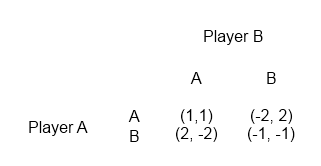
\includegraphics[scale=1.0]{PrisonersDilemma}
	\caption{Prisoner's Dilemma}
\end{figure}

If players A and B play with individual rationality, then they will each chose strategy B, as it dominates their strategy A. The result in this is case would be BB (-1, -1). However, this is not a Pareto optimal outcome, since AA (1, 1) would have been a better outcome for both players. So we see then, in fact, that paradoxically if they were to play their dominated strategies the collective and individual outcomes would be improved.

The question then, is how can non-cooperative players, who are not in communication (and thus cannot know what the other player will choose), resolve this paradox?

\subsection{N-Person Prisoner's Dilemma}

An N-person Prisoner's Dilemma game is characterized as any game in which each of $n$ players has two strategies, call them C and D, such that:

\begin{enumerate}[label=\roman{*})]
\item for every player, D is a dominant strategy, and
\item if all players choose D, all will be worse of than if all players had chosen C.
\end{enumerate}

We leave it as an exercise for the reader to examine the N-person game below, applying conditions i) and ii) to observe the Prisoner's Dilemma paradox.

\begin{figure}[H]
	\centering
	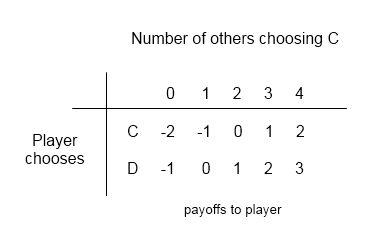
\includegraphics[scale=1.0]{NPersonDilemma}
	\caption{N-Prisoner's Dilemma}
\end{figure}

\section{Model of Professional Sports Drafts}

In order to analyze the draft system, it needs to be converted into a mathematical model. The draft system is used by various sports leagues in the United States, such as football and basketball, to organize the introduction of new players into the league. In order to promote a fair balance in talent between teams, the team that had the worst win-loss ratio in the previous season receives the first position in the draft. Each team takes a turn selecting a player in successive rounds until the pool of prospective players has been exhausted. The paper models the draft scenario by simplifying it into a non-zero sum sequential selection model, using $n$ teams and $kn$ players. In this way, teams make choices until each team has received $k$ players. The paper makes the following assumptions:

\begin{enumerate}

	\item{\em Strict preferences and partial ordering.} Each team has a strict preference ordering on the players in the draft, which induces a partial ordering on the sets of players which it might receive in the draft. This partial ordering is done by pairwise comparison. It is worth noting that there might be scenarios in which a team may have to make a judgment between sets which are incomparable by pairwise comparison. This assumption rules out more complicated drafting strategies such as, "I want this quarterback only if I can also get this pass receiver."

	\item{\em Self-interest.} The assumption is made that each team chooses their ordering in order to improve its own position and not to hurt other teams. 

	\item{\em Independence.} Each team makes their selections independently; there are no coalitions or hidden agreements.

	\item{\em Complete Information.} The assumption is made that each team knows the other teams preference orderings. The paper asserts that this may not be as outlandish an assumption as it might first appear, as teams now have extensive access to data regarding the players and the other teams current rosters. However, this is a very strong assumption, especially since the rest of the discussion relies upon this shared knowledge.

\end{enumerate}

\section{Two Teams Scenarios}

The simplest scenario for a draft is two teams. The paper begins by exploring this scenario with a pool of four players. 

\begin{figure}[H]
	\centering
	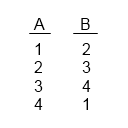
\includegraphics[scale=1.0]{TwoTeams}
	\caption{Two player draft with a four player pool}
\end{figure}

The straightforward way for the draft to proceed is with each team selecting the best available player each round. The paper refers to such decisions as being {\em sincere} selections. If each team follows a sincere strategy then the outcome is as follows:

\begin{figure}[H]
	\centering
	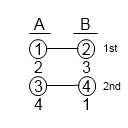
\includegraphics[scale=1.0]{TwoTeamsSincere}
	\caption{Sincere Choices}
\end{figure}

If we take assumption four into account, that each team knows the other teams preference orderings, we observe that it may be possible for teams to make {\em sophisticated} selections which will improve their outcome. For example, observe that team B places the least value on player 1. With this in mind, team A could defer selecting this player until the second round of selections ensuring that they will get player 2 first and then player 1 in the second round.

\begin{figure}[H]
	\centering
	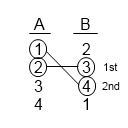
\includegraphics[scale=1.0]{TwoTeamsSophisticated}
	\caption{Sophisticated Choices}
\end{figure}

When both teams utilize their sophisticated choices, neither team could be assured of a better outcome by making different choices or strategies given the assumptions of the model. This outcome is referred to as the {\em sophisticated outcome}, which is the result of individually optimal play by both teams.

There exists an algorithm, presented by Kohler and Chandrasekaran\cite{kohler71}, which produces the optimum play outcome for a two team scenario in which each team is making sequential choices based upon complete information about each other's preferences. In their original presentation Kohler and Chandrasekaran prove that the resulting choice strategy is optimal for both teams. The proof begins by assuming that the method is optimal for a selection game involving two teams and two players. The proof then continues inductively on the number of players in order to show that it is optimal for $n$ players.

Having established that there exists and algorithm by which to calculate optimal choice strategies, the paper then turns to exploring whether these choice strategies are Pareto optimal. We begin by establishing a precise notion of Pareto optimality based upon the partial-ordering and self-interest assumptions. An allocation of players is said to be Pareto optimal with respect to pairwise comparison if there is no different allocation in which either team gets the same players, or prefers either allocation of players by pairwise comparison. This leads to the theorem that; if there are two teams, then the sophisticated outcome, as given by the Kohler and Chandrasekaran algorithm, is always Pareto optimal with respect to pairwise comparison. The theorem is proven by contradiction, in that the algorithm picks the next best choice in a bottom-up manner, so the best choice should always have been already taken in each step.

The paper concludes that for the two-team scenario the situation is rather pleasing in that there exists an efficient algorithm which can calculate the outcome obtained by individual optimal play, which is in fact, Pareto optimal. In the two-team scenario, no Prisoner's Dilemma can arise.

\section{Three or more teams}

The paper then considers the following situation with three teams and six players:

\begin{figure}[H]
	\centering
	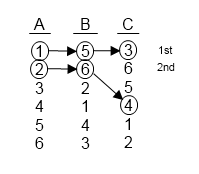
\includegraphics[scale=1.0]{ThreeOrMoreSincere}
	\caption{Sincere Choices}
\end{figure}

Using this game scenario the authors theorize that for any number of teams, the sincere outcome is always Pareto optimal with respect to pairwise comparison. However, although the paper proves that this theorem holds, it is also observed that the sincere choices are not optimal play. When the play is optimal, and the players are making their sophisticated choices, a Prisoner's Dilemma situation arises however, with each player receiving a strictly worse outcome than in the sincere scenario.

\begin{figure}[H]
	\centering
	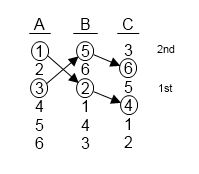
\includegraphics[scale=1.0]{ThreeOrMoreSophisticated}
	\caption{Sophisticated Choices}
\end{figure}

Based upon this observation, the paper then establishes the theorem that if there are three or more teams, then optimal play (i.e. the sophisticated choices) may lead to an outcome which is not Pareto optimal by pairwise comparison. In fact, such an outcome may be strictly worse than the sincere outcome for all teams. This bizarre situation, in which teams playing their sophisticated choices results only in damaging their own outcome, is referred to by the authors as the {\em paradox of player selection}. One notes that in the above scenario, the only choice made sophisticatedly is A's first choice, after which all choices are made in the same manner as would be sincerely, demonstrating how one choice can destroy the Pareto optimality.

As all teams are now in a worse position, it seems possible that they could trade players in a manner such that Pareto optimality could be restored. However, further consideration reveals that this is not possible through a sequence of mutually advantageous two-way trades, and that in fact no mutually advantageous two-way trade is possible in the sophisticated outcome scenario. Without outside mediation, it seems unlikely that a three-way cyclical trade could be organized. The authors conclude that, under the assumptions of the paper, there is only one modification which can prevent the paradox of player selection. This leads to the theorem that if there are three or more teams, and teams are following optimal drafting strategies, a team may do better by occupying a later position in the draft. The following example is provided to illustrate:

\begin{figure}[H]
	\centering
	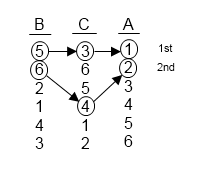
\includegraphics[scale=1.0]{ThreeOrMoreSincereAndSophisticated}
	\caption{Sincere and Sophisticated Choices}
\end{figure}

We note that team A does better when it chooses later in the draft. Indeed, we also see in this example that teams B and C have also improved their outcome. This results in a strange situation, in which the first-priority team, according to the drafting rules, actually would prefer to choose last, and in fact it would be to the shared benefit of all the teams to allow such a scenario. Given this seemingly odd modification the outcome is now, in fact, actually once again Pareto optimal.

\section{Remedies to the prisoners dilemma in sports drafts}

Finally, the authors show that it would be difficult if not impossible to enforce that teams use sincere choices. Furthermore, the paper illustrates the problems involved in the design of an algorithm that could theoretically find optimal selections and arranges trades that result in Pareto optimality. 

\begin{enumerate}

	\item{\em Algorithmic Complexity} An algorithm would have to traverse the entire sequential game tree in order find optimal play. Given $n$ teams and $kn$ players, the running time for such an algorithm would be $O(kn^{n})$, which is exponential and could be computationally innefficient.

	\item{\em Incomparable Allocations} Due to the limitations of pairwise comparison (assumption two in the model), the algorithm would not be aware of preferential information between incomparable allocations, hindering its ability to arrive at a unique sophisticated outcome.

	\item{\em Existence} A unique sophisticated outcome might not exist. (This is analogous to how players in a matrix game might not have any dominant strategies.)

	\item{\em Non-unique Trading Solutions} Once, and if, a unique outcome is found, there may be several ways to arrange the trades, making the algorithm less deterministic and more arbitrary in its results.

\end{enumerate}

Based upon these investigations the authors conclude that there is no feasible way to eliminated the pathology of the Prisoner's Dilemma from the current drafting scheme. More promisingly however, the authors provide examples of potentially fair player distribution schemes such as modified bidding or "marriage algorithms" which would even take into account player preferences for certain teams. 

\section{Implications}

Since being published, this paper has been cited in several game theory and economics textbooks \cite{straffin93}\cite{thomas03}\cite{roth92} as a real-world example of the Prisoner's Dilemma. Furthermore, this research was used in developing auctioning models and examining inefficiencies in the traditional modes of sequential bidding, as well as in designing fair agendas for Ireland and Denmark's political voting \cite{oleary05}  to avoid sequential assignment problems. 
However, we do make the observation that the assumptions made in this paper are quite strong. Specifically, the requirement that preference lists be constructed prior to the drafting process beginning precludes dynamic ranking lists. This rules out scenarios such as a team only preferring a certain player contingent upon getting a matching player (i.e. only wanting a quarterback with the matching receiver.) In reality, teams would likely deviate from their original preference ordering as the draft progressed, to take into account when a player becomes unavailable. Others \cite{fry07} have attempted to tackle the sports drafting problem by slightly deviating from Bram and Straffin's model, tending towards a more realistic set of assumptions that more accurately model the National Football League (NFL).
We make the observation that the concepts presented in this paper closely tie in with the Fair Division (or Cake-Cutting) problem, which has been fertile ground for a plethora of mathematical research on achieving Pareto optimality, amongst other fairness criteria.

\section{Conclusion}

While the current drafting system used in many professional sports leagues in the United States can be shown to be optimal for two teams it is, in the much more likely scenario, unable to produce satisfactory results for a league with three or more teams. This is due to the Prisoner's Dilemma that occurs when teams pursue their individual self-interests by making sophisticated choices about which players to select first. In pursuing their rational strategies the teams actually prevent the Pareto optimal solution from being attainable. Further, the drafting model examined in the paper is so flawed that it seems infeasible to make any easy modification that would resolve the situation and restore Pareto optimality. However, alternative fair distribution schemes are presented by both the original paper and in other literature cited by this report. Given the pervasive nature of Prisoner's Dilemma type scenarios it is promising to find that such alternative schemes exist. 

\pagebreak[4]
\bibliography{MATH5607ReportBib}{}
\bibliographystyle{plain}

\end{document}